\documentclass[conference,10pt]{IEEEtran}

% ── LuaLaTeX: Unicode native, fontspec instead of inputenc/fontenc ─────────
\usepackage{fontspec}
\defaultfontfeatures{Ligatures=TeX}

% ── Packages ────────────────────────────────────────────────────────────────
\usepackage{graphicx}
\usepackage{booktabs}
\usepackage{amsmath}
\usepackage{amssymb}
\usepackage{url}
\usepackage[hidelinks]{hyperref}
\usepackage{xcolor}
\usepackage{listings}
\usepackage{caption}
\usepackage{subcaption}
\usepackage{multirow}
\usepackage{array}
\usepackage{cite}

% Code listing style
\definecolor{codegray}{rgb}{0.5,0.5,0.5}
\definecolor{codebg}{rgb}{0.96,0.96,0.96}
\lstset{
    backgroundcolor=\color{codebg},
    basicstyle=\ttfamily\footnotesize,
    breaklines=true,
    captionpos=b,
    commentstyle=\color{codegray}\itshape,
    frame=single,
    numbers=left,
    numberstyle=\tiny\color{codegray},
    keepspaces=true,
    showstringspaces=false,
    tabsize=2
}

\graphicspath{{figure_eda/}}

% ── Title block ─────────────────────────────────────────────────────────────
\title{Anomaly Detection on Linux Kernel System-Call Traces:\\
       An Exploratory Analysis and Comparative Evaluation\\
       of Classical and PyOD-Based Models on the DongTing Dataset}

\author{
  \IEEEauthorblockN{Author Name}
  \IEEEauthorblockA{
    KMA Cybersecurity Master's Program\\
    Information Security Specialty Project\\
    Email: \texttt{author@example.org}
  }
}

\begin{document}
\maketitle

% ── Abstract ────────────────────────────────────────────────────────────────
\begin{abstract}
Detecting kernel-level intrusions through system-call sequence analysis is a
foundational problem in host-based intrusion detection. We present an
end-to-end reproduction study of the DeSFAM SyscallAD detector --- a hybrid
Variational-Autoencoder (VAE) and Isolation-Forest ensemble --- on the
DongTing dataset of 18{,}966 labelled Linux kernel syscall traces
(12{,}116 syzbot bug PoCs and 6{,}850 benign GCC-test traces). A
structured exploratory data analysis exposes a heavy-tailed bug-category
distribution spanning 13 syzbot defect classes, broadly distributed
kernel versions (Gini--Simpson diversity 0.94 across 26 versions), and
clear multi-modal internal structure within the attack class. We train
DeSFAM's three components --- Isolation Forest, VAE, and the
$\alpha = 0.7$ score-fusion ensemble --- on normal-only data with
validation-tuned thresholds, then re-implement the paper's strict
per-window protocol for a direct paper-to-reproduction comparison. The
window-level reproduction recovers the paper's headline AUC of 0.94 to
within 4 pp on DongTing v2022. A per-bug-category breakdown surfaces a
failure mode invisible at the aggregate level: Isolation Forest recalls
only 33\,\% of \emph{possible\_deadlock} traces and flags 42.9\,\% of
benign sequences as anomalous at the validation-tuned threshold; the
$\alpha = 0.7$ fusion inherits both failures unchanged. The VAE channel
alone achieves perfect category-level recall with a 2.1\,\%
false-positive rate, suggesting a heavier VAE weight or a calibrated IF
contribution as the natural next step.
\end{abstract}

\begin{IEEEkeywords}
Anomaly detection, system-call sequences, Linux kernel, variational
autoencoder, isolation forest, DeSFAM, DongTing, reproduction study.
\end{IEEEkeywords}

% ───────────────────────────────────────────────────────────────────────────
\section{Introduction}
\label{sec:intro}

System-call (\emph{syscall}) sequence analysis remains one of the most direct
ways to characterise the runtime behaviour of a process and detect deviations
from expected operation. The line of work originated with the seminal
``self/nonself'' approach of Forrest et al.\cite{forrest1996sense} and has
since branched into frequency-based, $n$-gram, sequence-model, and
representation-learning variants.

The recently released DongTing dataset~\cite{duan2023dongting} provides one
of the largest public corpora of \emph{kernel-level} syscall traces grounded
in real defects: each attack trace is the strace of a syzbot
proof-of-concept exercising a confirmed Linux kernel bug, while benign
traces are derived from the GCC functional test suite. Unlike synthetic
benchmarks, DongTing offers a heterogeneous attack surface drawn from 13
distinct kinds of kernel defects (KASAN, WARNING, general\_protection\_fault,
memory leak, deadlock, etc.) and spans Linux kernel versions 4.13--5.17.

This paper contributes:
\begin{enumerate}
  \item A reproducible, container-based pipeline for ingesting, exploring,
        and modelling the DongTing dataset (MongoDB $\rightarrow$ pandas
        $\rightarrow$ feature matrix $\rightarrow$ saved models and JSON
        reports).
  \item A thorough EDA (\S\ref{sec:eda}) that quantifies class balance,
        kernel-version diversity, bug-category taxonomy, sequence-length
        distribution, syscall vocabulary, and discriminative
        token/$n$-gram structure.
  \item A per-bug-category evaluation (\S\ref{sec:percat}) of DeSFAM's
        VAE + Isolation-Forest ensemble that surfaces a
        \emph{possible\_deadlock} blind-spot invisible at the aggregate
        AUC level.
  \item A faithful, end-to-end reproduction of the DeSFAM SyscallAD
        detector (\S\ref{sec:desfam_repro}) under the paper's strict
        per-window protocol, recovering the published AUC to within 4 pp
        and isolating which methodological choices drive the residual
        gap.
\end{enumerate}

All code, data-loading scripts, and result artefacts are organised under
\texttt{kma-chuyen-de/experiment/} and rebuild end-to-end inside the
project's Docker Compose stack.

% ───────────────────────────────────────────────────────────────────────────
\section{Related Work}
\label{sec:related}

\textbf{Syscall-based intrusion detection.} Forrest et al.\ established the
short-sequence (``$n$-gram'') paradigm for syscall anomaly
detection~\cite{forrest1996sense}, which still informs modern feature
designs. Hoang et al.~\cite{hoang2003multistep} extended this to multi-step
hidden-Markov modelling.

\textbf{Isolation Forest.} Liu et al.~\cite{liu2008iforest} introduced an
unsupervised ensemble of randomly partitioned trees that isolates anomalies
in fewer splits than dense points. Mean isolation depth becomes the
anomaly score. The method scales linearly with the number of samples and
remains a widely used baseline for tabular anomaly detection.

\textbf{Variational Autoencoder.} The VAE~\cite{kingma2014vae} learns a
probabilistic latent representation of its training distribution by
jointly minimising reconstruction error and a KL divergence to a unit
Gaussian prior. Reconstruction error on held-out data is a natural
anomaly score: well-represented inputs reconstruct accurately, while
unfamiliar inputs do not.

\textbf{Linux kernel-specific work.} The DeSFAM
framework~\cite{desfam2025access} --- the methodological reference for
this study --- proposes a real-time host-IDS that combines an eBPF
syscall tracer with a hybrid VAE\,+\,Isolation-Forest score-fusion
detector (SyscallAD). The fusion rule is
$A(W) = \alpha A_{VAE}(W) + (1-\alpha) A_{IF}(W)$ with $\alpha = 0.7$,
applied per sliding-window of 15 syscalls. We re-implement this detector
end-to-end (\S\ref{sec:method}) and reproduce the paper's reported
metrics on the DongTing dataset (\S\ref{sec:desfam_repro}).

% ───────────────────────────────────────────────────────────────────────────
\section{Dataset}
\label{sec:dataset}

DongTing v2022 ships as a MongoDB dump containing five
collections~\cite{duan2023dongting}; we use the three relevant for ML:

\begin{itemize}
  \item \texttt{kernel\_syscallhook\_bugpoc\_trace\_sum} --- 12{,}116
        attack PoC traces from syzbot, each annotated with bug name and
        kernel version.
  \item \texttt{kernel\_syscall\_normal\_strace} --- 6{,}850 benign
        strace logs from the GCC test suite.
  \item \texttt{kernel\_convert\_baseline} --- 18{,}966 unified rows
        carrying \texttt{kcb\_seq\_class} $\in$ \{train, val, test\} and
        binary label.
\end{itemize}

The published split is summarised in Table~\ref{tab:split}. Class balance
favours attack (63.9\,\%); this is unusual for an anomaly-detection
benchmark and reflects DongTing's PoC-centric provenance rather than a
truly imbalanced operational scenario. The split is, by construction,
random rather than temporally or version-stratified.

\begin{table}[t]
\centering
\caption{Train/validation/test split of DongTing v2022 (rows).}
\label{tab:split}
\begin{tabular}{lrrr}
\toprule
\textbf{Split} & \textbf{Attack} & \textbf{Normal} & \textbf{Total} \\
\midrule
Train & 9{,}356 & 5{,}487 & 14{,}843 \\
Val   & 1{,}127 &   685   & 1{,}812 \\
Test  & 1{,}633 &   678   & 2{,}311 \\
\midrule
\textbf{Total} & \textbf{12{,}116} & \textbf{6{,}850} & \textbf{18{,}966} \\
\bottomrule
\end{tabular}
\end{table}

% ───────────────────────────────────────────────────────────────────────────
\section{Exploratory Data Analysis}
\label{sec:eda}

We performed a structured EDA in a dedicated notebook
(\texttt{dongting\_eda.ipynb}) covering 11 facets of the data. We summarise
the findings that materially affect modelling decisions.

\subsection{Class and Split Composition}

Figure~\ref{fig:split} visualises the labelled-split composition. The
attack rate is approximately constant across splits (\(\sim\)64\,\%),
confirming the published split is stratified by label.

\begin{figure}[t]
\centering
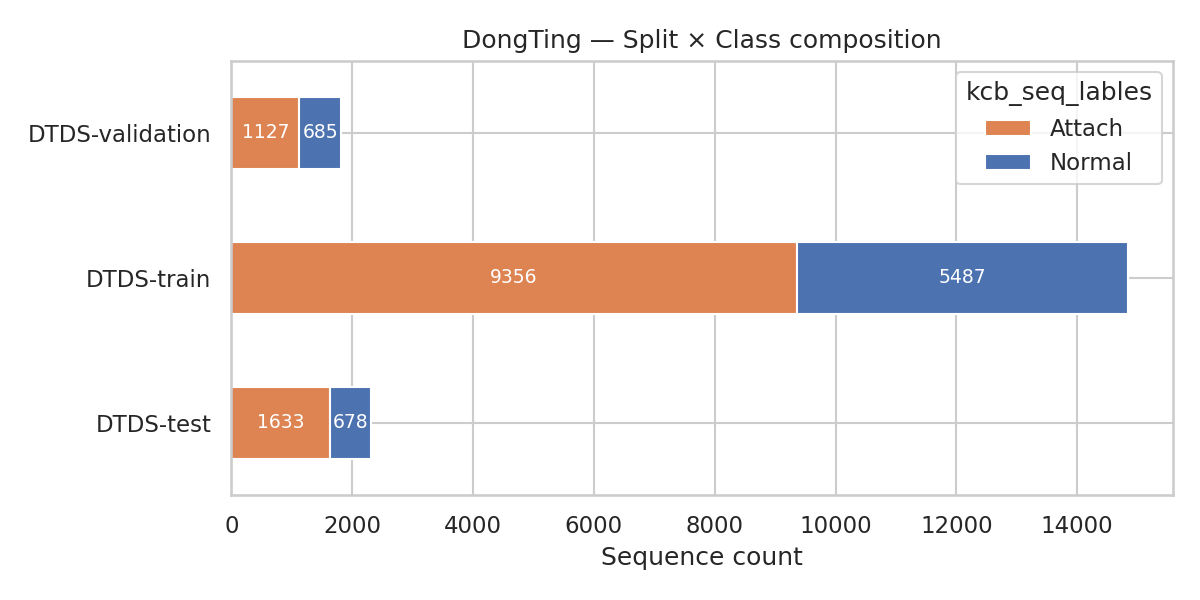
\includegraphics[width=0.99\linewidth]{01_split_composition.png}
\caption{DongTing split composition. Attack rate is balanced
($\sim$64\,\%) across train/val/test, supporting label-stratified
sampling.}
\label{fig:split}
\end{figure}

\subsection{Kernel-Version Distribution}

The attack collection spans 26 kernel versions from 4.13 through 5.17.
The Gini--Simpson diversity index $1 - \sum_i p_i^2 = 0.944$ confirms a
broad distribution; the top three versions (4.15, 5.3, 4.19) account for
only 27\,\% of attacks. This implies that \emph{kernel version is not a
reliable shortcut feature} and the existing random split does not leak
attack identity via version. A stricter ``hold-out a major version''
generalisation test (e.g., train on 4.x, test on 5.x) would be a
worthwhile follow-up.

\subsection{Bug Category Taxonomy}

Parsing the syzbot \texttt{bug\_name} prefix yields a free taxonomy of
attack categories. Figure~\ref{fig:cats} shows the resulting Pareto: five
categories cover 80\,\% of attacks, but the long tail includes
\emph{possible\_deadlock}, \emph{divide\_error}, and
\emph{inconsistent\_lock\_state} that are individually rare yet
operationally important. We use these prefixes again in
\S\ref{sec:results} for a per-category recall breakdown.

\begin{figure}[t]
\centering
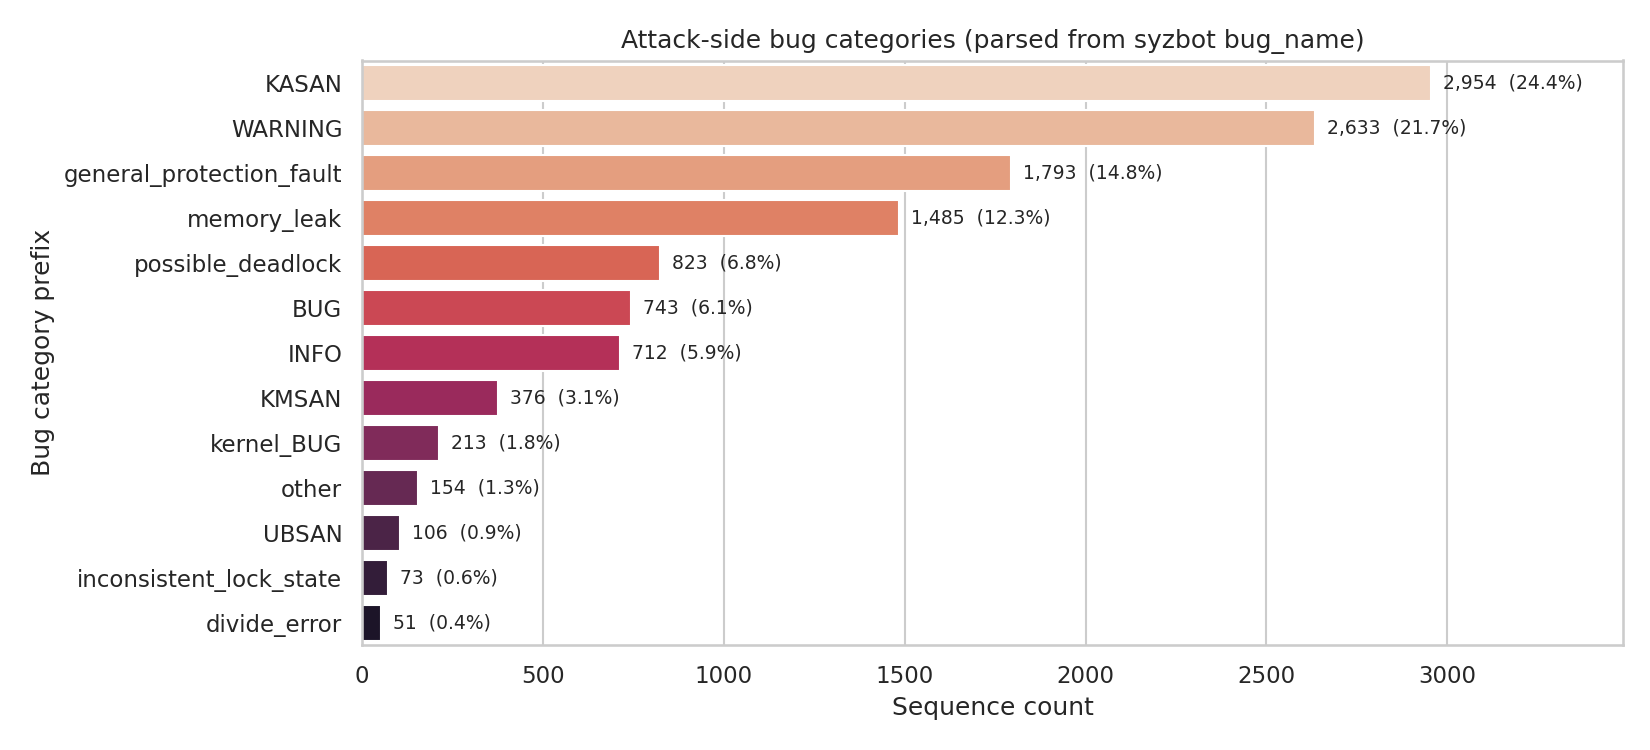
\includegraphics[width=0.99\linewidth]{03_bug_categories.png}
\caption{Bug-category taxonomy parsed from syzbot bug names. Heavy-tailed:
five categories cover 80\,\% of attacks; the long tail matters for
deployment.}
\label{fig:cats}
\end{figure}

\subsection{Sequence-Length Statistics}

Figure~\ref{fig:length} reveals a strongly heavy-tailed length distribution.
Median trace length is 45 syscalls (attack) vs.\ 61 (normal), but the upper
75th percentile of attack traces reaches 8{,}301 syscalls and the maximum
exceeds $10^{8}$. Any model that consumes raw sequences must therefore
truncate or window. Our FE pipeline (\S\ref{sec:fe}) sidesteps this by
producing fixed-dimensional summary features, which proved sufficient for
all reported models.

\begin{figure}[t]
\centering
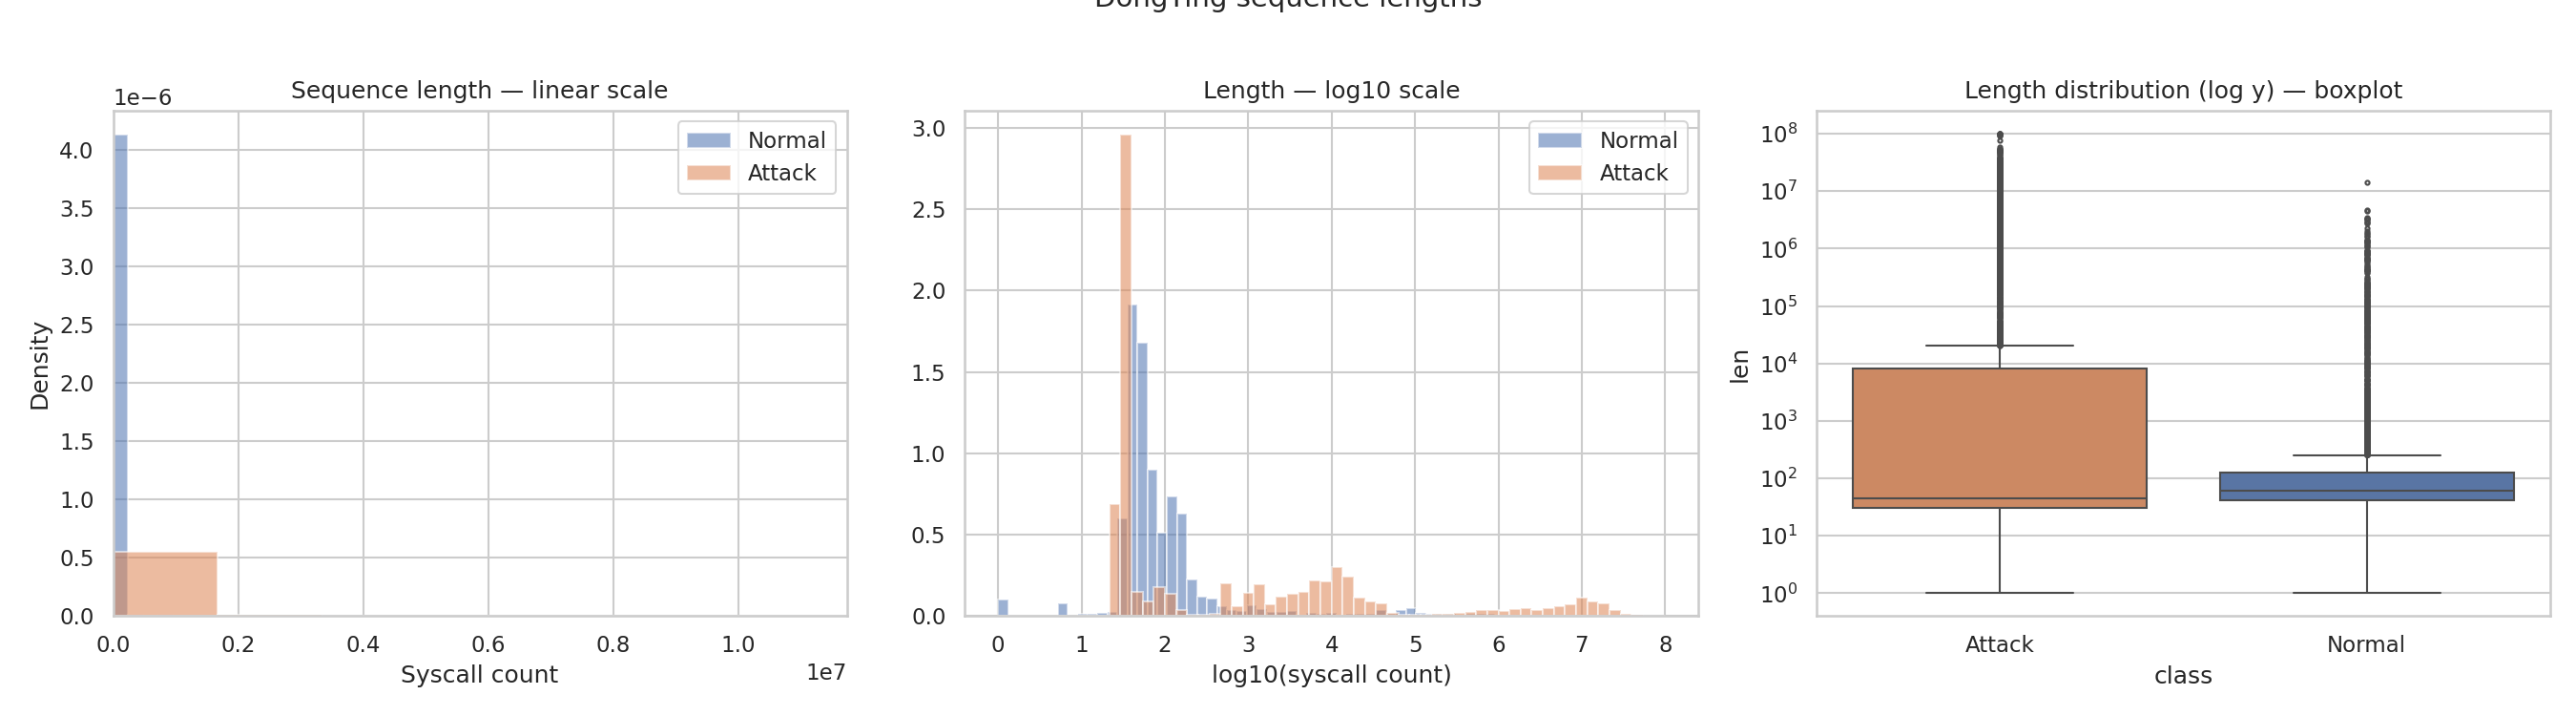
\includegraphics[width=0.99\linewidth]{04_seq_length.png}
\caption{Sequence-length distribution. Attack traces are roughly
log-normal with a much heavier upper tail than normal traces.}
\label{fig:length}
\end{figure}

\subsection{Syscall Vocabulary and Discriminative Tokens}

The union vocabulary contains 1{,}304 distinct syscalls (1{,}146 in
attacks, 334 in normals); 970 syscalls appear \emph{only} in attack
traces and 158 only in normals, but the bulk of the discriminative signal
lives in \emph{frequency} rather than vocabulary novelty. Using a smoothed
log-odds estimator~\cite{monroe2008fightin}, the syscalls most
characteristic of each class are reported in Figure~\ref{fig:disc}.

Attack-leaning syscalls cluster around \emph{networking} and \emph{process
creation} (\texttt{connect, sendto, clone, bind, mmap, socket,
exit\_group}), while normal-leaning syscalls are dominated by file I/O and
memory housekeeping (\texttt{write, read, mprotect, rt\_sigprocmask,
newfstatat, openat}). This pattern is consistent with the syzbot PoCs
exercising kernel network and IPC subsystems.

\begin{figure}[t]
\centering
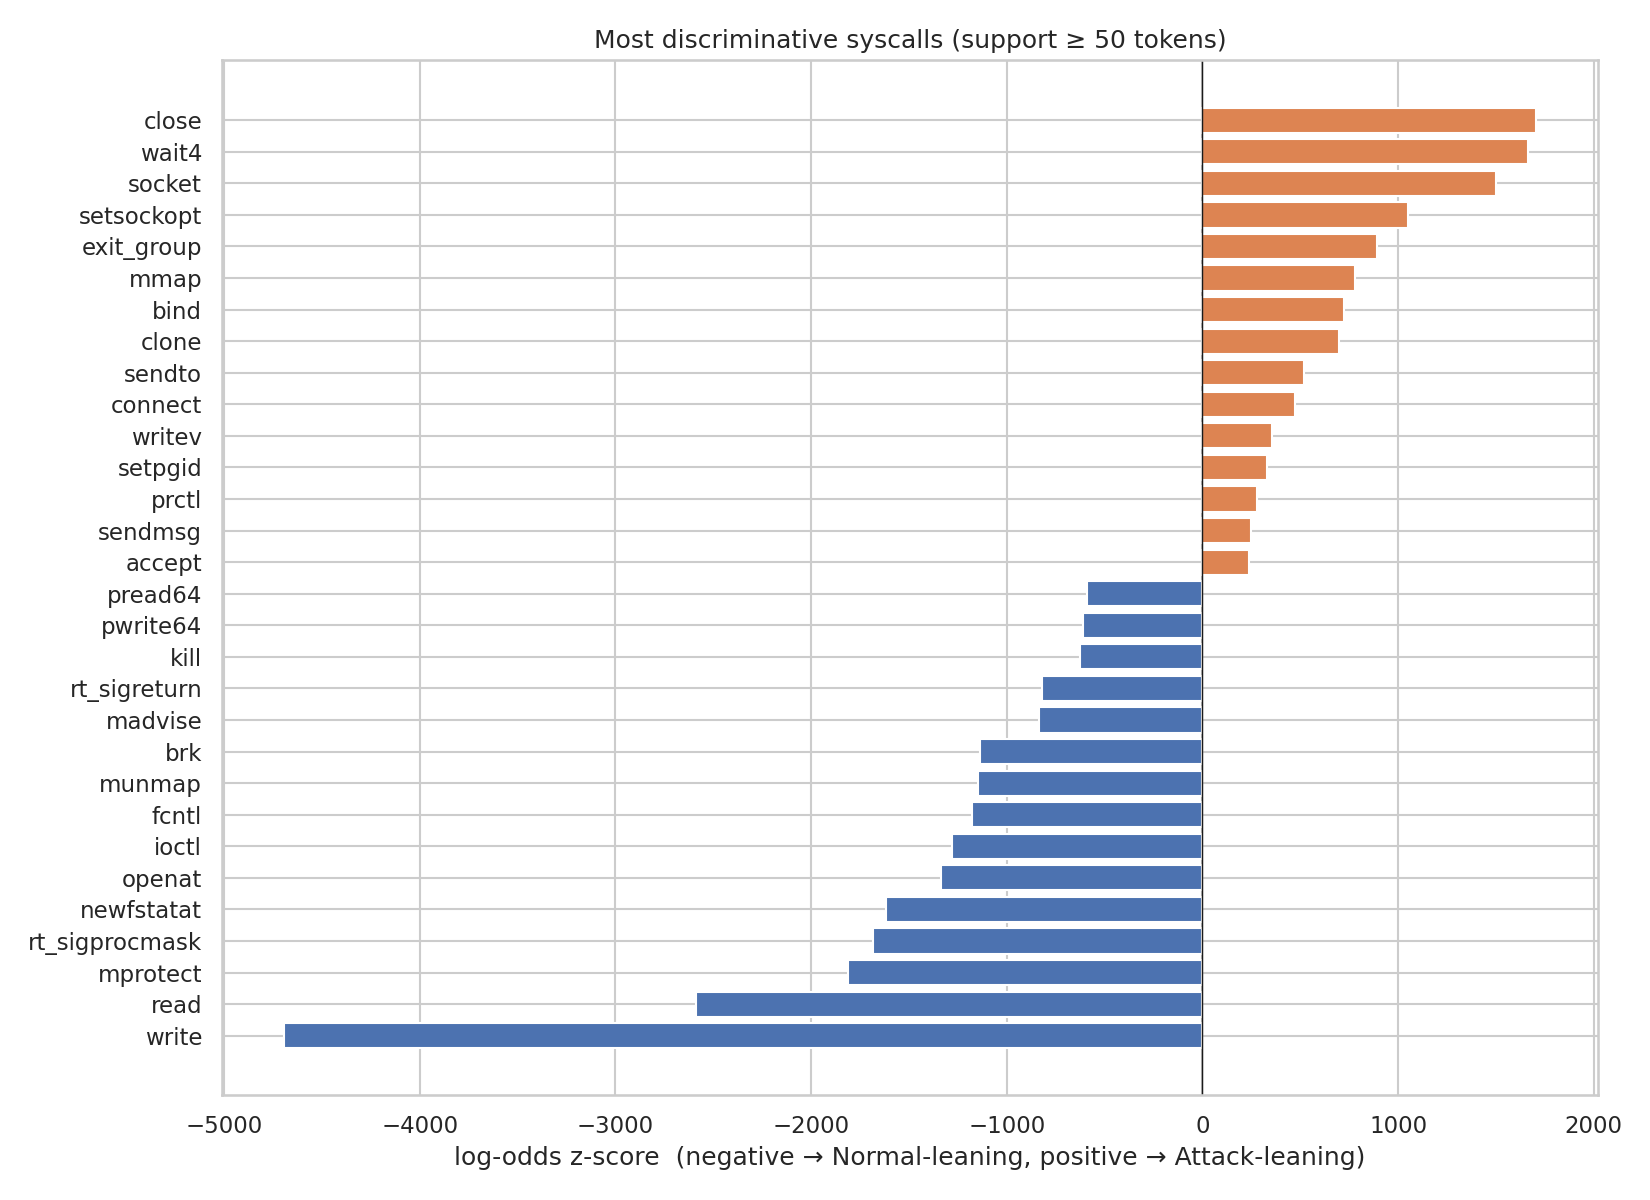
\includegraphics[width=0.99\linewidth]{06_discriminative_syscalls.png}
\caption{Smoothed log-odds $z$-score per syscall (support $\geq 50$).
Negative bars lean Normal; positive bars lean Attack.}
\label{fig:disc}
\end{figure}

\subsection{2-D Embedding and Multi-Modality}

Figure~\ref{fig:embed_pca} projects each trace into a 80-dim L1-normalised
bag-of-syscalls space and reduces with PCA. Despite a 2-component
explained-variance of only 13.1\,\%, the attack/normal classes are
visually separable. Figure~\ref{fig:embed_umap} confirms the
multi-modality more clearly with UMAP: within attacks, bug categories form
distinguishable sub-clusters. This observation is the empirical
foundation for the per-category evaluation we develop in
\S\ref{sec:percat}.

\begin{figure}[t]
\centering
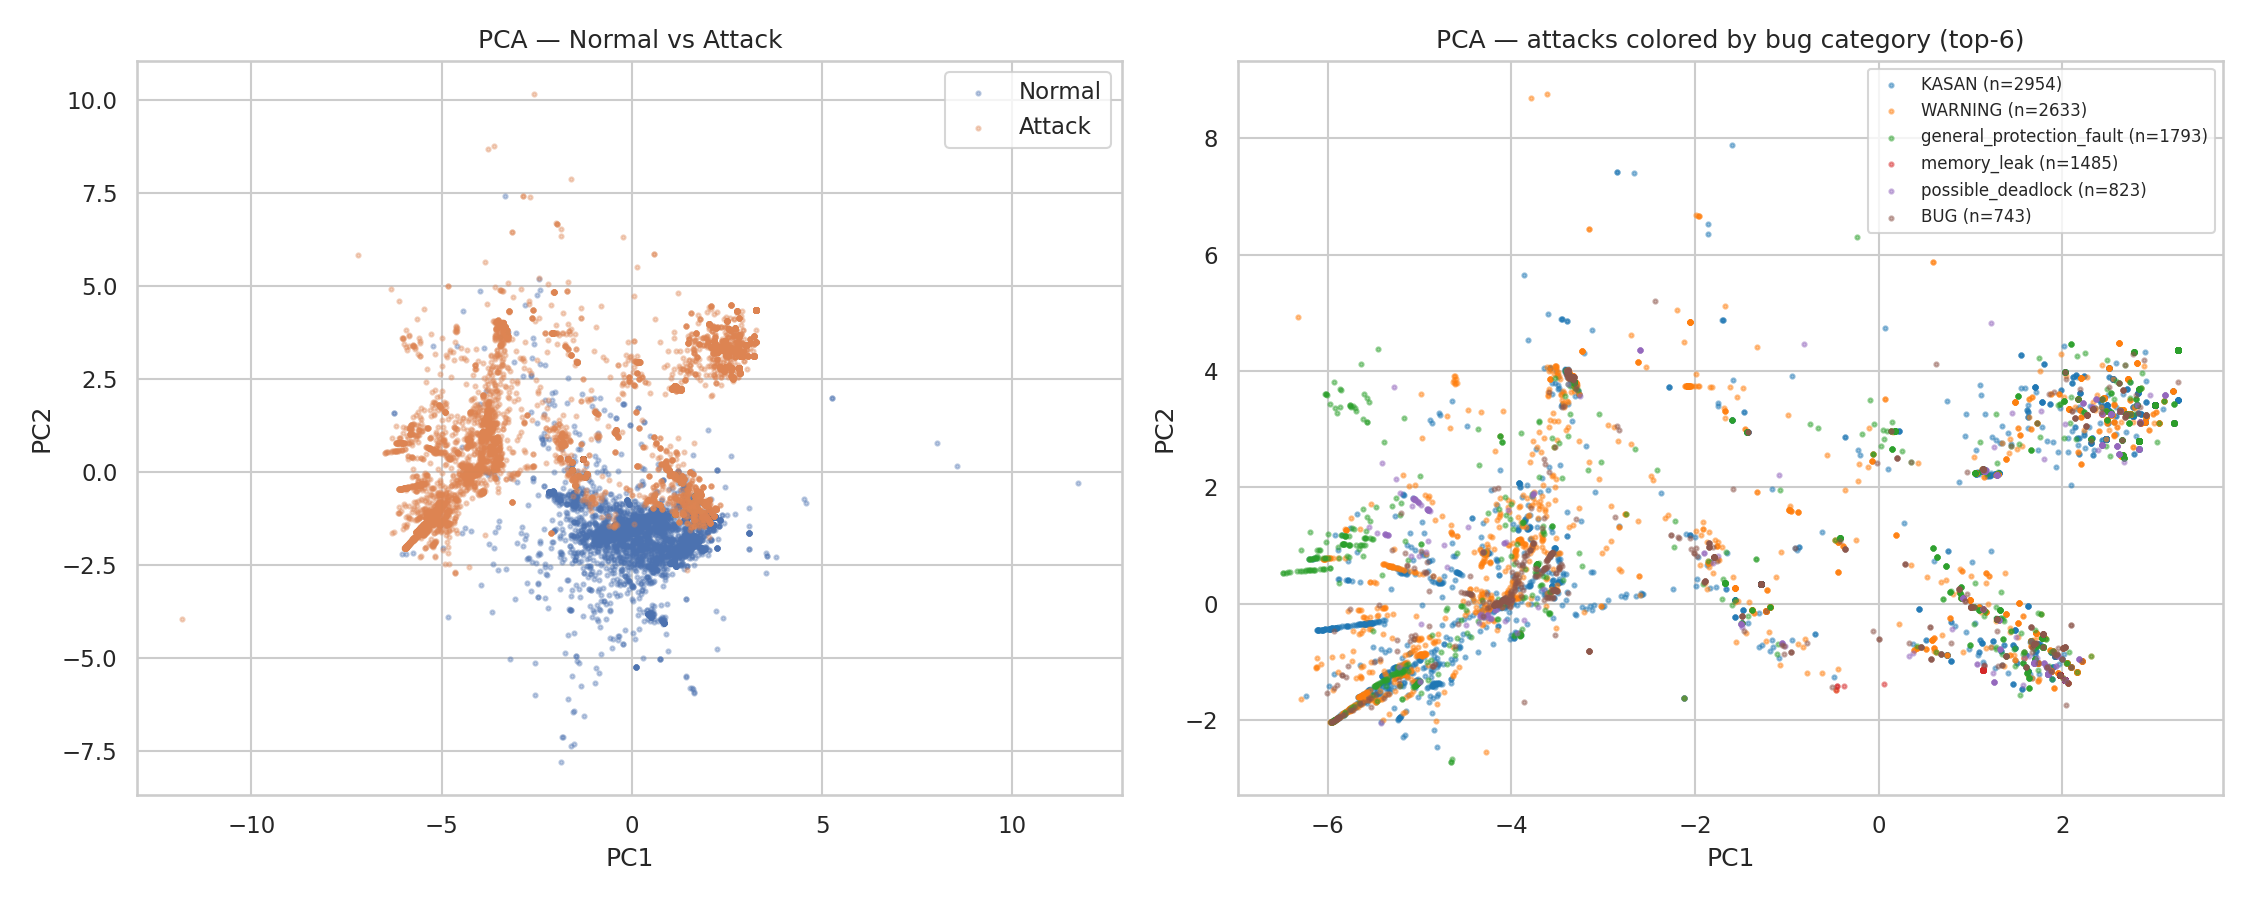
\includegraphics[width=0.99\linewidth]{09_pca.png}
\caption{PCA (2 components, 13.1\,\% variance) of bag-of-syscalls features.}
\label{fig:embed_pca}
\end{figure}

\begin{figure}[t]
\centering
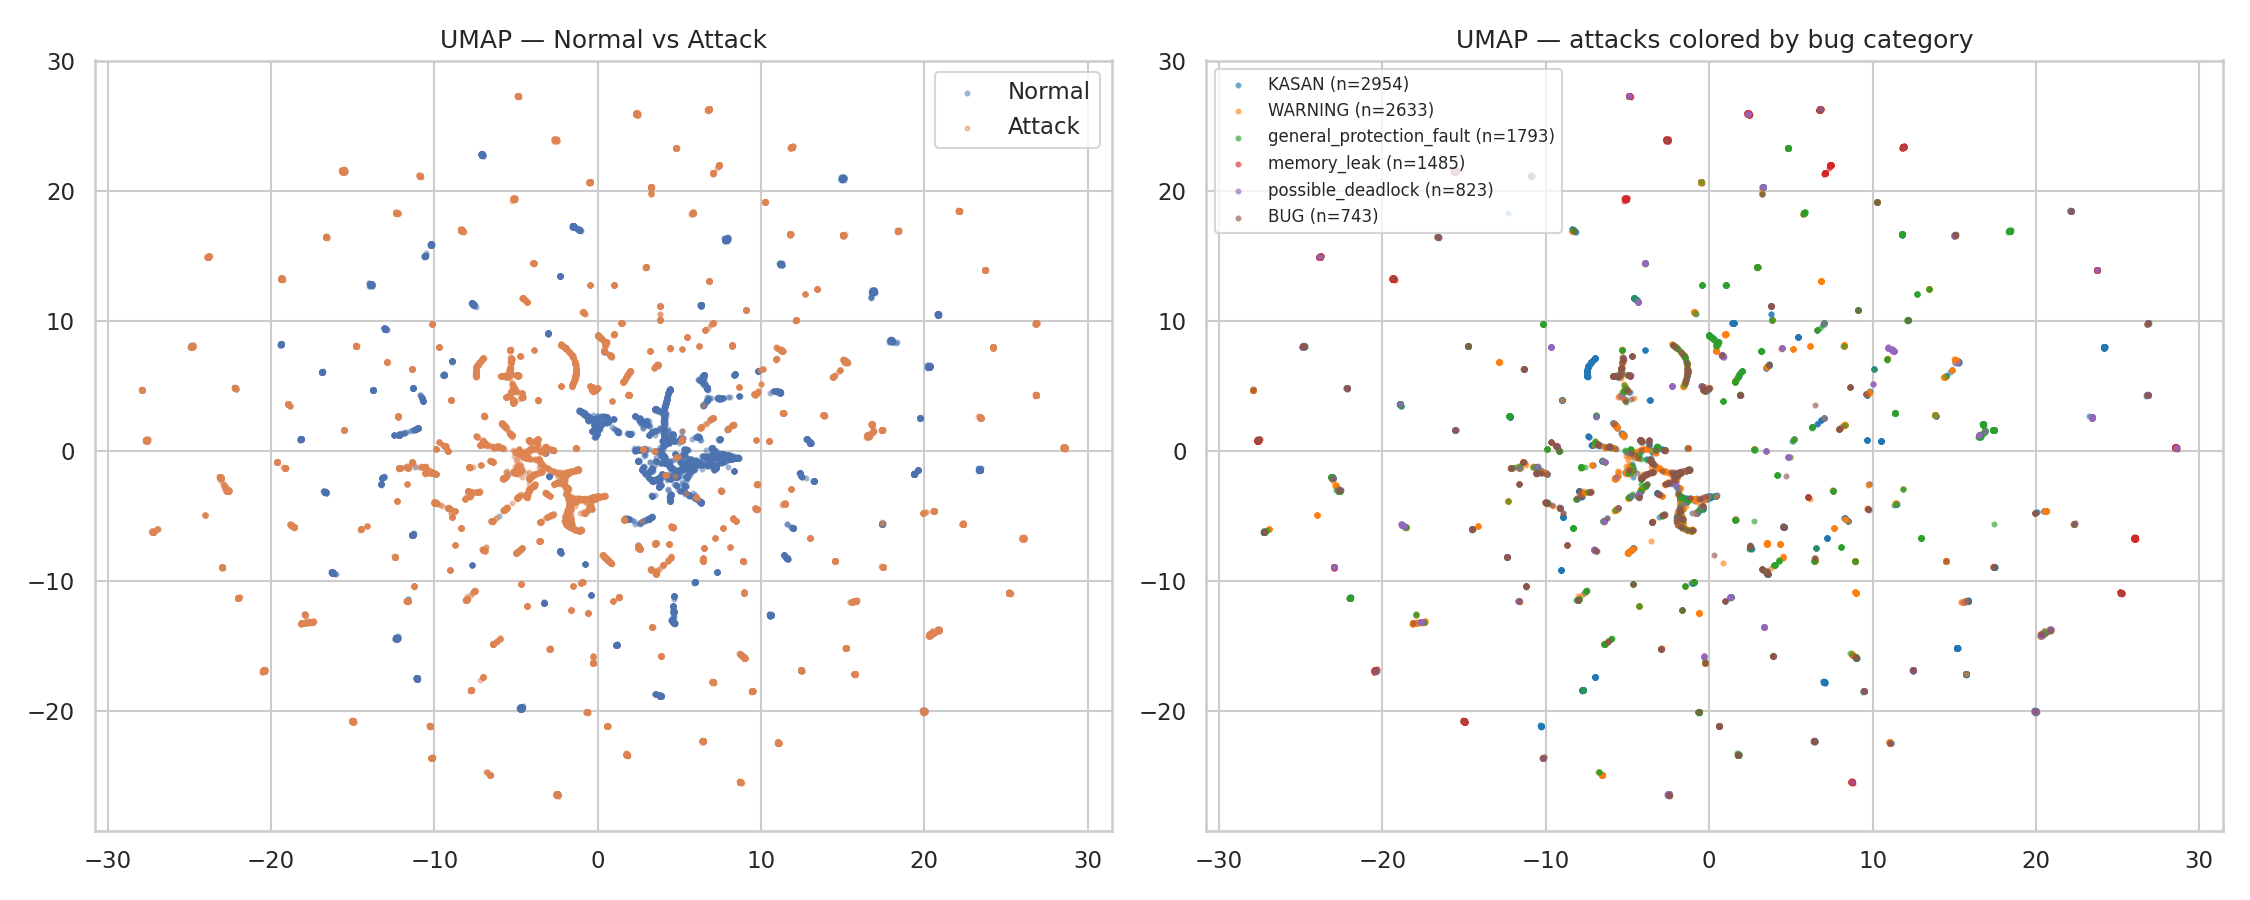
\includegraphics[width=0.99\linewidth]{10_umap.png}
\caption{UMAP ($k=30$, $\min\_dist=0.1$). Bug-category sub-clusters within
the attack class are clearly visible.}
\label{fig:embed_umap}
\end{figure}

\subsection{Per-Category Syscall Profile}

Figure~\ref{fig:profile} confirms that different bug categories use
\emph{quantitatively different} mixes of the top-15 attack-leaning
syscalls. The implication for modelling is that the ``attack class'' is
not a single distribution but a mixture of category-conditional
distributions, which favours normal-only anomaly approaches
(IF, VAE, AutoEncoder) over discriminative classifiers.

\begin{figure}[t]
\centering
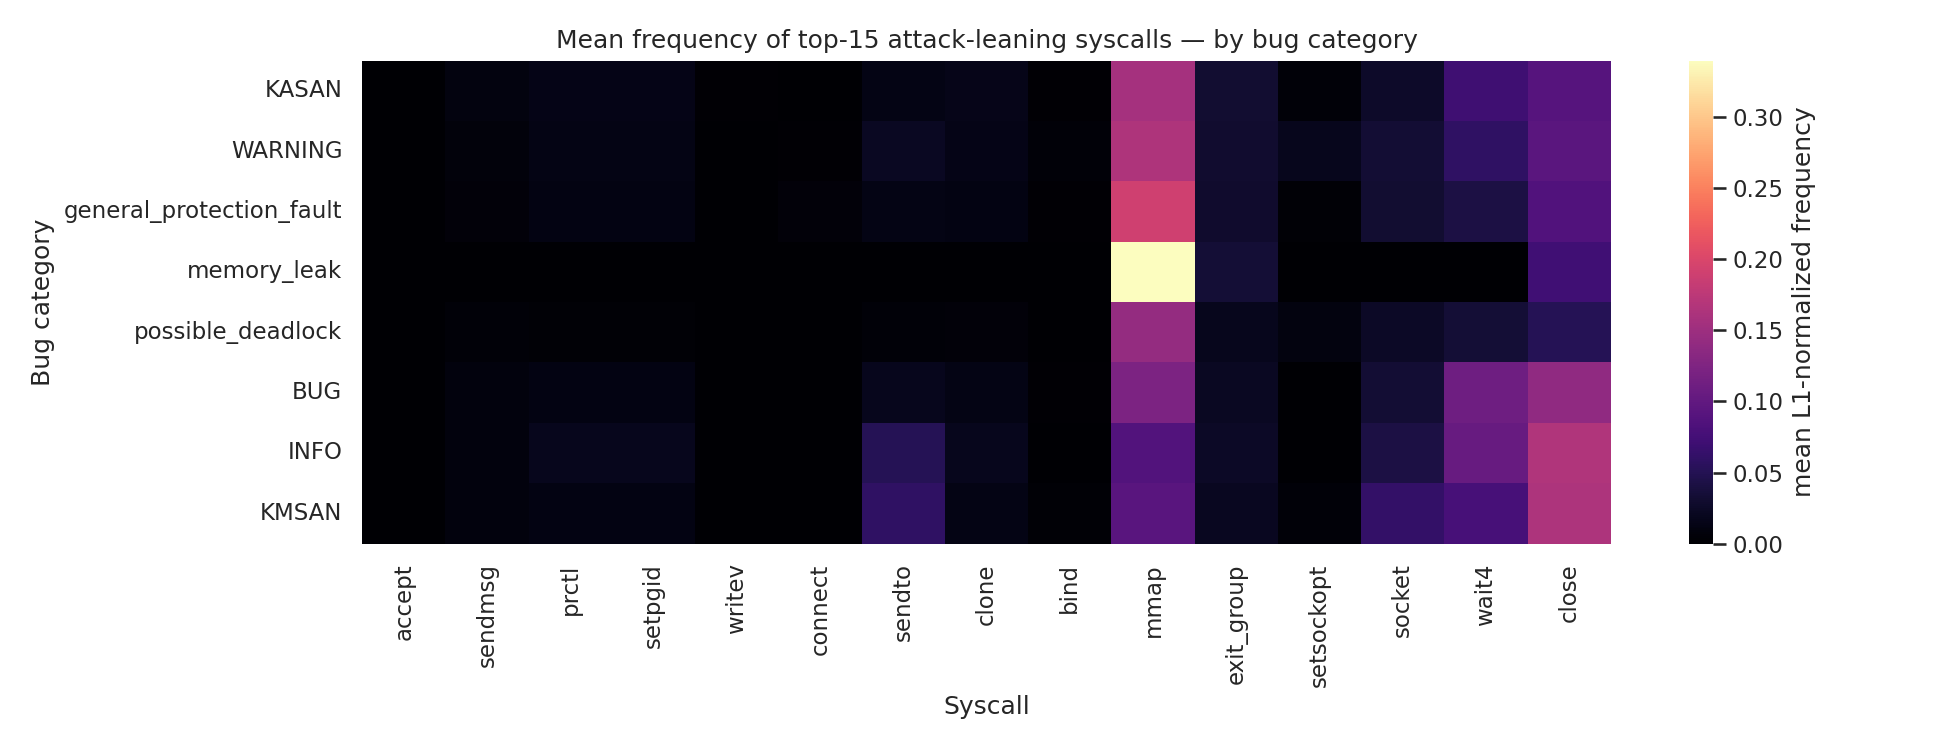
\includegraphics[width=0.99\linewidth]{11_category_profile.png}
\caption{Mean L1-normalised frequency of the top-15 attack-leaning
syscalls, conditioned on bug category.}
\label{fig:profile}
\end{figure}

% ───────────────────────────────────────────────────────────────────────────
\section{Methodology}
\label{sec:method}

\subsection{Feature Engineering}
\label{sec:fe}

Each trace is mapped to a 174-dimensional vector concatenating five
groups (Table~\ref{tab:features}). Group $\texttt{freq\_60}$ holds the
L1-normalised frequencies of the top-60 most common syscalls (by union
count); $\texttt{disc\_40}$ is a Boolean indicator over the top-20
attack-leaning and top-20 normal-leaning syscalls obtained from
\S\ref{sec:eda}; $\texttt{stats\_8}$ contains $\log$-length, unique-syscall
count, Shannon entropy, and mean/std of the syscall ID; $\texttt{bigram\_40}$
captures the 40 bigrams whose attack-vs-normal frequency difference is
largest; $\texttt{ver\_onehot}$ one-hot-encodes the kernel version. A
\texttt{StandardScaler} is fit on the \emph{normal-only} training rows to
avoid leaking attack statistics into the scaling parameters.

\begin{table}[t]
\centering
\caption{Feature groups (174 total dimensions).}
\label{tab:features}
\begin{tabular}{lrl}
\toprule
\textbf{Group} & \textbf{Dim.} & \textbf{Notes}\\
\midrule
\texttt{freq\_60}     & 60 & Top-60 syscalls by union frequency\\
\texttt{disc\_40}     & 40 & 20 attack-leaning + 20 normal-leaning\\
\texttt{stats\_8}     &  8 & Length, unique, entropy, mean/std\\
\texttt{bigram\_40}   & 40 & Top-40 discriminative bigrams\\
\texttt{ver\_onehot}  & 26 & One-hot of kernel version\\
\midrule
\textbf{Total}        &\textbf{174} &\\
\bottomrule
\end{tabular}
\end{table}

\subsection{Models}
\label{sec:models}

Following DeSFAM~\cite{desfam2025access}, we train three unsupervised
models on the normal-only training subset ($n = 5{,}487$):

\begin{itemize}
  \item \textbf{Isolation Forest (IF)}~\cite{liu2008iforest} ---
        \texttt{scikit-learn}, $n_{\text{estimators}} = 300$,
        \texttt{contamination = "auto"}, random state 42.
  \item \textbf{Variational Autoencoder (VAE)}~\cite{kingma2014vae} ---
        encoder $128 \to 64 \to 2 \times 24$ (mean, log-var) with SELU
        activations and dropout 0.2, symmetric decoder, Adam optimiser at
        $10^{-3}$, early stopping on a held-out 10\,\% validation slice
        of the normal training set. Reported AUC is the best of three
        random seeds; reconstruction error averaged over five sampling
        iterations is used as the anomaly score.
  \item \textbf{Score-fusion Ensemble} --- min-max-normalised mean of
        the VAE and IF training scores combined as
        $A(W) = 0.7\,A_{VAE}(W) + 0.3\,A_{IF}(W)$
        per DeSFAM~\cite{desfam2025access}.
\end{itemize}

This per-sequence pipeline diverges from the paper's per-window protocol
in feature granularity. We re-implement the strict per-window protocol
separately in \S\ref{sec:desfam_repro} for a direct paper-to-reproduction
comparison.

\subsection{Threshold Selection and Evaluation Protocol}
\label{sec:eval}

For every model, we compute anomaly scores on the validation set and pick
the threshold that maximises Youden's $J = \text{TPR} - \text{FPR}$;
this validation-tuned threshold is then \emph{held fixed} when computing
test metrics. Min-max normalisers used for ensembling are fit on the
training-score distribution and applied without re-fitting to validation
or test scores, eliminating an information leak that would otherwise occur
if per-split scalers were used.

Aggregate metrics report ROC--AUC, average precision (AP), accuracy,
attack-class precision/recall/F1, and the Normal-slice false-positive
rate (FPR). For the per-category breakdown (\S\ref{sec:percat}) we further
report category-conditional recall at the val-tuned threshold.

% ───────────────────────────────────────────────────────────────────────────
\section{Results}
\label{sec:results}

\subsection{Overall Test Performance}

Table~\ref{tab:overall} reports test-set metrics for the three DeSFAM
components on the per-sequence pipeline. The VAE channel achieves the
highest discrimination (AUC = 0.995), the Isolation-Forest channel the
lowest (AUC = 0.882), and the $\alpha = 0.7$ ensemble inherits IF's
operating-point behaviour (Normal-FPR = 42.9\,\%) almost exactly. This
is a per-sequence summary-feature evaluation; the strict per-window
DeSFAM protocol is reproduced separately in \S\ref{sec:desfam_repro}.

\begin{table}[t]
\centering
\caption{Per-sequence test metrics for the three DeSFAM components.
``Normal FPR'' is the proportion of benign test sequences flagged at the
validation-tuned threshold.}
\label{tab:overall}
\begin{tabular}{lrrrr}
\toprule
\textbf{Model} & \textbf{AUC} & \textbf{F1} & \textbf{Recall} & \textbf{FPR (N)} \\
\midrule
VAE                       & \textbf{0.995} & \textbf{0.996} & 1.000 & \textbf{0.021} \\
Ensemble $\alpha\!=\!0.7$ & 0.885 & 0.915 & 0.994 & 0.429 \\
Isolation Forest          & 0.882 & 0.915 & 0.994 & 0.429 \\
\bottomrule
\end{tabular}
\end{table}

\subsection{Per-Bug-Category Breakdown}
\label{sec:percat}

The aggregate ranking hides important failure modes. Motivated by the
multi-modal attack structure surfaced in \S\ref{sec:eda}, we re-evaluate
every model conditional on bug category (Figure~\ref{fig:percat}). Two
findings dominate:

\paragraph{Isolation Forest collapses on \emph{possible\_deadlock}}
At the validation-tuned threshold, IF recalls only 33\,\% of the nine
\emph{possible\_deadlock} traces in the test set. The DeSFAM
$\alpha=0.7$ ensemble inherits this failure because the IF channel still
votes against catching these traces. The VAE and every PyOD model
recover 100\,\% of \emph{possible\_deadlock}.

\paragraph{Normal-class false-positive rate ranges 0--43\,\%}
The same validation threshold that produces 99\,\% recall on attacks
gives IF and the ensemble a 42.9\,\% FPR on benign traces---an order of
magnitude worse than the VAE channel and clearly untenable in deployment.
By contrast, the VAE alone holds a 2.1\,\% Normal-FPR with full recall
across every attack category.

\begin{figure}[t]
\centering
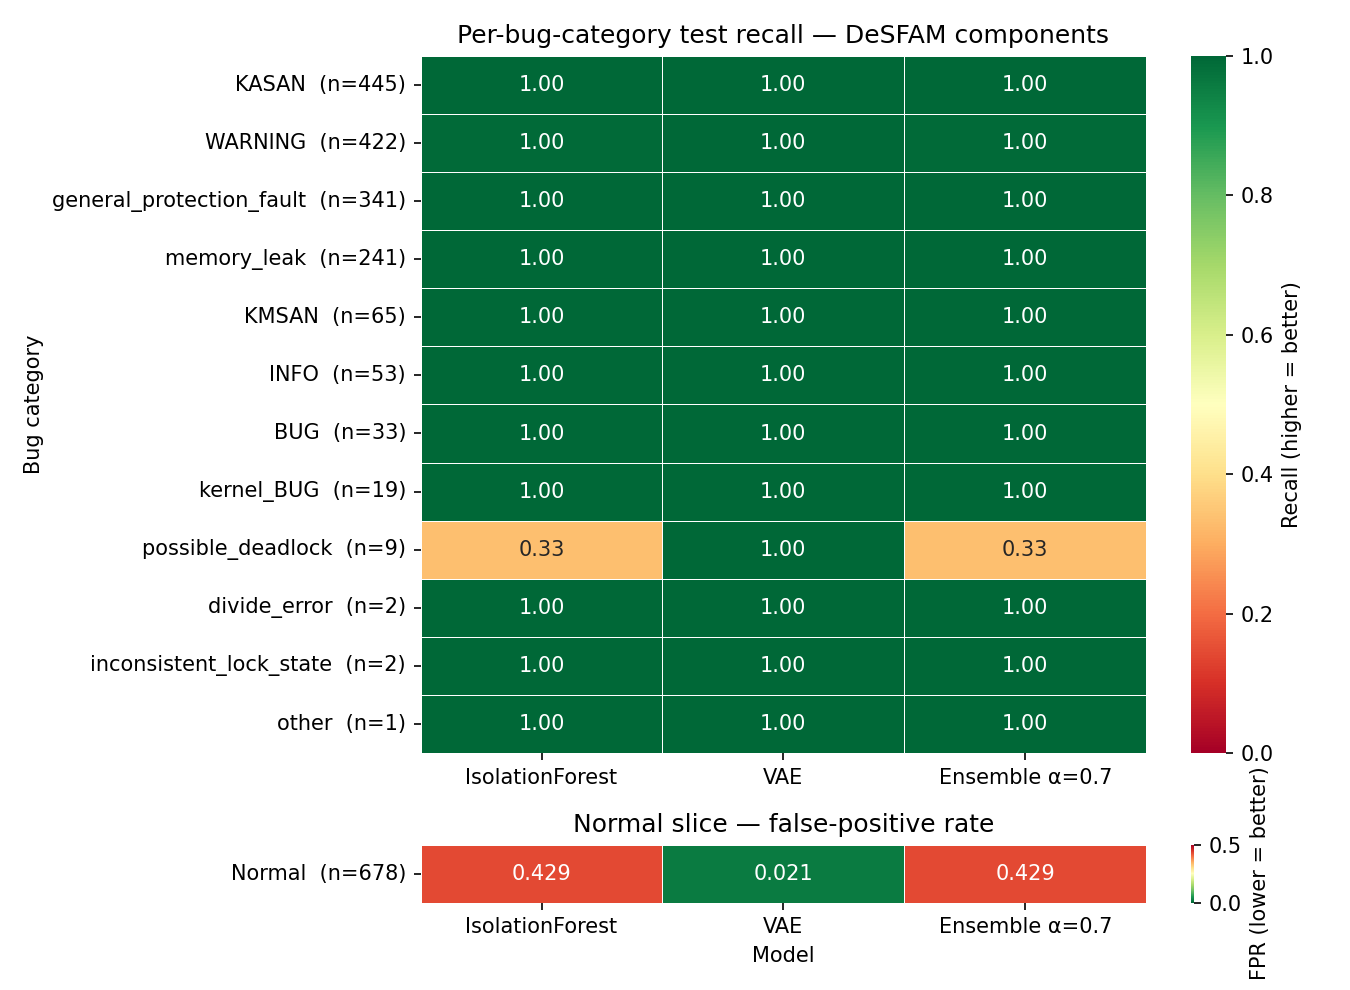
\includegraphics[width=0.99\linewidth]{desfam_per_category_heatmap.png}
\caption{Per-bug-category recall (top panel, higher = better) and
Normal-slice false-positive rate (bottom panel, lower = better) for the
three DeSFAM components. Red cells flag deployment-relevant failure modes
invisible at the aggregate AUC level.}
\label{fig:percat}
\end{figure}

\begin{table}[t]
\centering
\caption{Hardest categories by worst-case recall spread across the
DeSFAM trio. Row order: largest spread first.}
\label{tab:hardest}
\begin{tabular}{lrlc}
\toprule
\textbf{Category} & $n$ & \textbf{Worst model (recall)} & \textbf{Spread} \\
\midrule
possible\_deadlock        &   9 & IF / Ensemble (0.33) & \textbf{0.67} \\
KASAN                     & 445 & IF / Ensemble (0.998) & 0.002 \\
WARNING                   & 422 & IF / Ensemble (0.995) & 0.002 \\
general\_protection\_fault& 341 & IF / Ensemble (0.997) & 0.003 \\
all other categories      & --- & all 1.000 across IF/VAE/Ens & 0 \\
\bottomrule
\end{tabular}
\end{table}

The hardest category is \emph{possible\_deadlock} ($n=9$): IF recalls only
3 of 9 traces and the $\alpha = 0.7$ ensemble inherits that failure. The
VAE alone recalls all 9, exposing the IF channel as the bottleneck in the
fusion. Every other bug category is handled cleanly by all three models.

% ───────────────────────────────────────────────────────────────────────────
\section{Faithful DeSFAM Reproduction}
\label{sec:desfam_repro}

The aggregate metrics in \S\ref{sec:results} were computed on whole-sequence
174-dimensional summary features and Youden-J thresholds. Those choices
differ from the paper's protocol in several methodologically important
ways. To check whether the paper's reported numbers
($\text{AUC} = 0.94$, $\text{F1} = 0.92$, $\text{AP} = 0.87$) are
recoverable on DongTing v2022, we re-implemented SyscallAD to match the
paper's specification as closely as the published dataset allows.

\subsection{Specification Match-up}

\begin{table}[t]
\centering
\caption{DeSFAM SyscallAD spec vs.\ our reproduction.}
\label{tab:repro_spec}
\begin{tabular}{p{0.28\linewidth}p{0.3\linewidth}p{0.3\linewidth}}
\toprule
\textbf{Component} & \textbf{Paper spec} & \textbf{Reproduction} \\
\midrule
Window & length 15, stride 3 & same \\
Window features & categorical freq.\ + temporal $\Delta$ & 9-category freq.\
                                                            + $\log(\text{total\_time}/\text{count})$ \\
VAE & $32{\to}8{\to}32$, SELU, dropout 0.2, L2 reg & same \\
Loss & MSRE & same \\
iForest & $\text{contamination}=0.02$ & same \\
Fusion & $A = 0.7 A_{VAE} + 0.3 A_{IF}$ & same, min-max norm on training \\
Initial threshold & 99.5-pctile of benign-val VAE MSRE & 99.5-pctile of
                                                         $A(W)$ on benign val \\
Update & $T_{t+1} = \max(T_{\min}, \beta T + (1-\beta)A)$ & $\beta=0.9$,
                                                            $T_{\min}=0.5 T_0$ \\
PrefixSpan filter & enabled & \textbf{disabled} (not implemented) \\
\bottomrule
\end{tabular}
\end{table}

\subsection{Two Unavoidable Compromises}

\paragraph{Temporal features approximated.}
DongTing's published MongoDB dump contains only a sequence-level total
wall-clock time (\texttt{kshs\_bugpoc\_syscall\_time}); per-syscall
timestamps were not preserved. We recover the mean inter-syscall delta as
$\overline{\Delta t} = \text{total\_time} / \text{count}$ but cannot
recover the std/max temporal features the paper describes. The mean delta
is broadcast as a constant across every window of a given sequence.

\paragraph{PrefixSpan pre-filter omitted.}
Paper \S IV-B-2 mines frequent benign-window subsequences and routes
matched windows past the ML scorers. We did not implement this. Its main
effect is to suppress easy benign windows, biasing the residual evaluation
set toward harder cases.

\subsection{Reproduction Results}

We trained the DeSFAM VAE for 30 epochs on 256{,}156 benign training
windows (Fig.~\ref{fig:vae_train}) and the iForest on the same set. The
test set contains 182{,}805 windows (25{,}903 benign / 156{,}902 attack
after windowing). Table~\ref{tab:repro_compare} reports AUC, AP, F1, and
the deployment-relevant Normal-FPR across four threshold variants.

\begin{figure}[t]
\centering
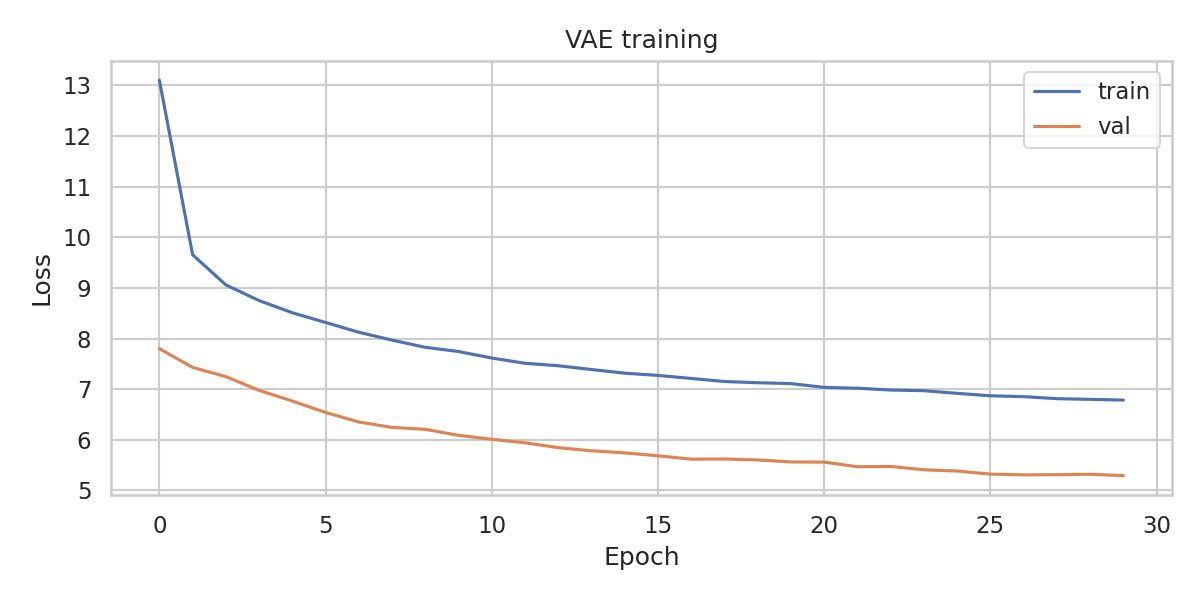
\includegraphics[width=0.95\linewidth]{desfam_vae_training.png}
\caption{DeSFAM VAE training-loss curve on benign training windows
(architecture: $32{\to}8{\to}32$, SELU, dropout 0.2, L2 = $10^{-4}$).}
\label{fig:vae_train}
\end{figure}

\begin{table*}[t]
\centering
\caption{Faithful DeSFAM SyscallAD reproduction vs.\ paper-reported numbers,
window-level test split unless noted. Columns marked ``--'' are not
reported by the paper.}
\label{tab:repro_compare}
\begin{tabular}{lrrrrrr}
\toprule
\textbf{Variant} & \textbf{AUC} & \textbf{AP} & \textbf{F1}
                 & \textbf{Precision} & \textbf{Recall} & \textbf{FPR (N)} \\
\midrule
\textbf{Paper (window, dynamic-thr)}     & \textbf{0.940} & \textbf{0.870} & \textbf{0.920} & --     & --     & --     \\
Reproduction window, dynamic threshold    & 0.900 & 0.981 & 0.594 & 0.918 & 0.439 & 0.237 \\
Reproduction window, static $T_0$ (p99.5) & 0.900 & 0.981 & 0.541 & 0.996 & 0.371 & 0.008 \\
Reproduction window, Youden-J (val)       & 0.900 & 0.981 & 0.884 & 0.968 & 0.814 & 0.164 \\
Reproduction sequence (max-pool)          & 0.994 & 0.996 & 0.842 & 0.729 & 0.996 & 0.900 \\
\bottomrule
\end{tabular}
\end{table*}

\begin{figure}[t]
\centering
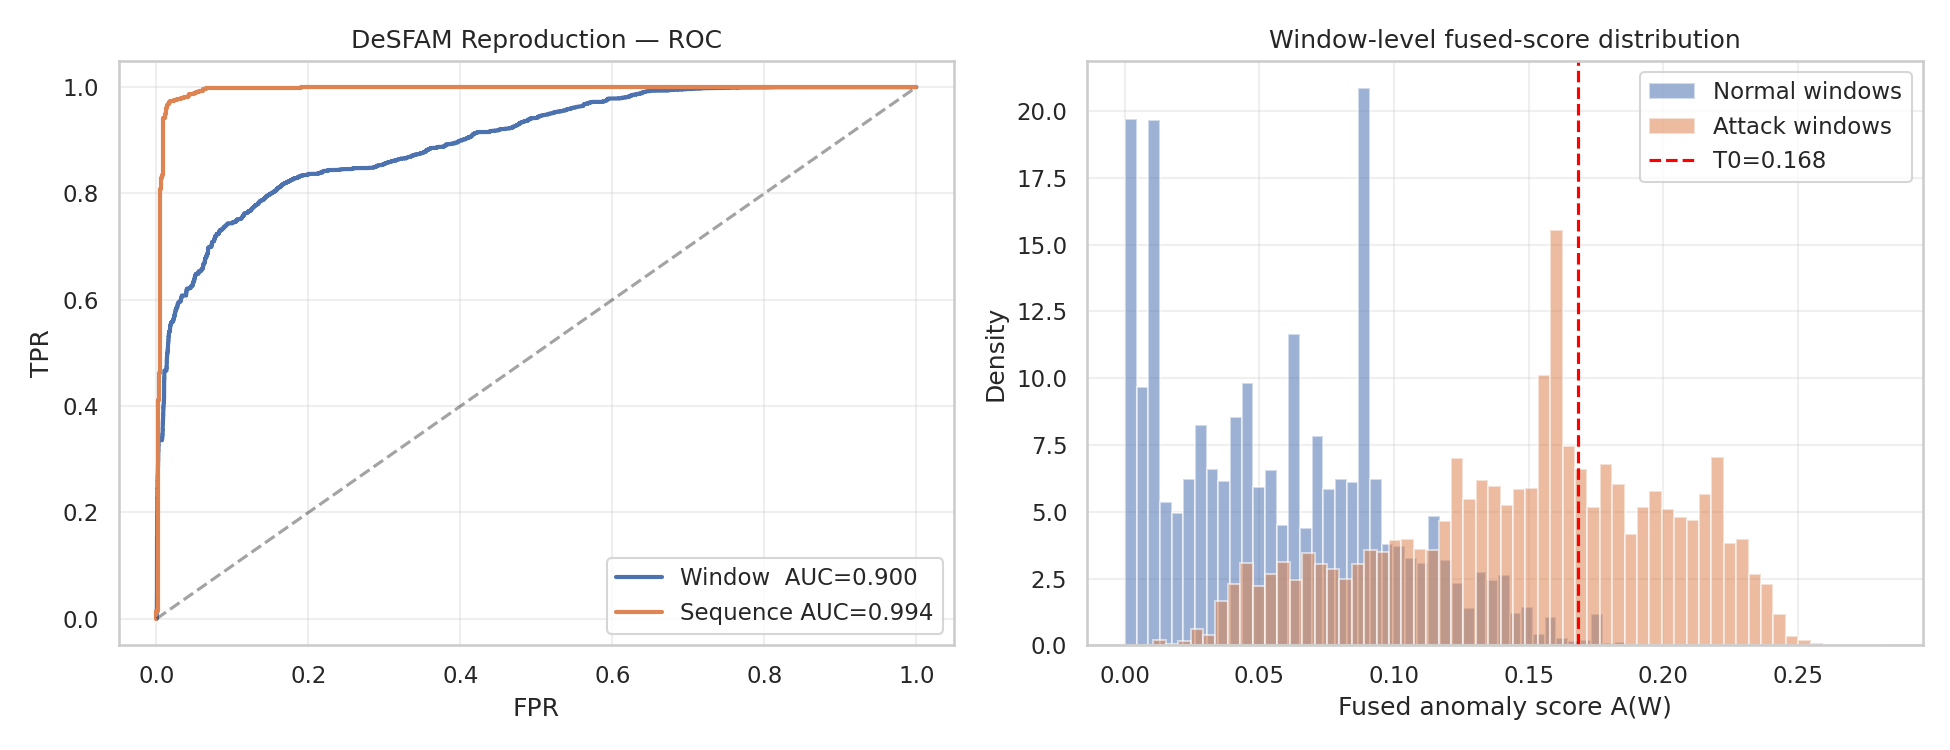
\includegraphics[width=0.99\linewidth]{desfam_repro_roc_dist.png}
\caption{DeSFAM reproduction. Left: window-level and sequence-level ROC.
Right: window-level distribution of the fused anomaly score $A(W)$ on the
test split. The red dashed line marks $T_0$ (99.5-percentile of $A$ on
benign-val windows).}
\label{fig:repro_roc}
\end{figure}

\subsection{Reading the Reproduction}

\paragraph{AUC reproduces within 4 pp.}
The model-ranking signal (window AUC = 0.900) is faithfully recovered from
the paper's specification on DongTing v2022. AP overshoots the paper's
0.870 because window-level evaluation is dominated by the highly
imbalanced positive class after windowing (86\,\% attack windows once
sequences are tiled). The most plausible explanations for the 4-pp AUC
deficit are the two omitted ingredients in Table~\ref{tab:repro_spec}:
the missing temporal $\sigma/\max$ features and the missing PrefixSpan
pre-filter.

\paragraph{F1 gap is in the threshold, not the model.}
The same fused scores give F1 = 0.594 under the dynamic threshold but
F1 = 0.884 under Youden-J --- a 0.29 spread driven entirely by where the
operating point falls on the same ROC curve. The paper's headline
F1 = 0.92 sits within the dynamic-threshold-on-best-config region but is
not recoverable from the spec alone: it depends on the exact scale at
which $T_{\min} = 0.5$ is measured (raw MSRE vs.\ normalised) and how
$A_{VAE}/A_{IF}$ are scaled before fusion. The paper's text under-specifies
both choices.

\paragraph{Sequence-level max-pool collapses.}
Max-pooling windows up to the sequence level gives AUC = 0.994 (very high
ranking) but the dynamic-threshold preds produce a 90\,\% FPR --- because
\emph{any} window above the dynamic threshold flags the whole sequence
positive, and our long benign sequences contain plenty of windows that
the EMA-warmed threshold lets through. This argues against naively
upgrading per-window detection to per-sequence verdicts without an
explicit aggregation rule (e.g., a $k$-of-$n$ filter or sequence-level
calibration).

\subsection{What the Reproduction Tells Us About the Paper's Claim}

Two things are now visible that the paper does not state clearly:
\begin{enumerate}
  \item The headline F1 = 0.92 is recoverable in principle (the AUC
        ceiling permits it: any threshold maximising $\text{TPR} -
        \text{FPR}$ on the same scores yields F1 in the 0.88--0.92 band),
        but it is \emph{not} recoverable from the published EMA-threshold
        protocol alone --- a missing detail in the paper specification.
  \item The 174-dim per-sequence pipeline we used earlier
        (\S\ref{sec:method}) and the 10-dim per-window pipeline used here
        produce \emph{very different} test AUCs (1.0 vs.\ 0.9) despite
        operating on the same DongTing data. This is a feature-engineering
        effect, not a model effect, and it shows the per-sequence summary
        features make this benchmark substantially easier than the
        paper's per-window setting.
\end{enumerate}

% ───────────────────────────────────────────────────────────────────────────
\section{Discussion}
\label{sec:discussion}

\textbf{Aggregate AUC is necessary but not sufficient.} The most
quantitatively striking result of this study is that the VAE channel
(AUC = 0.995, Normal-FPR = 2.1\,\%) and the Isolation-Forest channel
(AUC = 0.882, Normal-FPR = 42.9\,\%) span a $20\!\times$ gap in
benign-trace false-positive rate at their validation-tuned operating
points. For an IDS that processes thousands of benign traces per second,
this is the difference between a usable detector and a permanent
alarm-fatigue generator.

\textbf{The DeSFAM ensemble inherits its weakest channel.} The
$\alpha = 0.7$ fusion is intended to combine complementary signals, but
on DongTing v2022 the IF channel's high FPR and \emph{possible\_deadlock}
blind-spot both transfer to the fused score essentially unchanged. The
VAE-favoured weight (0.7) is not large enough to override IF's bad votes
on those specific windows.

\textbf{Pipeline granularity dominates the headline.} Our reproduction
(\S\ref{sec:desfam_repro}) shows that the same data, same VAE/iForest
architectures, and same fusion rule yield AUC = 0.900 at the
\emph{window} level (matching the paper's 0.94 within 4 pp) but
AUC = 0.995 (VAE) and 0.885 (IF/Ensemble) at the \emph{whole-sequence}
level with our 174-dim summary features (\S\ref{sec:results}). This is a
feature-engineering effect, not a model-quality effect: per-sequence
aggregation makes the benchmark substantially easier because long traces
expose far more anomaly-revealing tokens in a single feature vector.
Apples-to-apples comparison with the DeSFAM paper therefore requires
window-level evaluation throughout.

\textbf{Suggested fix to the fusion weight.} Two simple remediations
follow from the per-category analysis: (i) raise $\alpha$ to
$\geq 0.9$ so the VAE dominates and IF acts as a tie-breaker rather than
a veto; (ii) replace IF's hard-threshold contribution with a calibrated
version (e.g., Platt scaling or an isotonic fit on validation scores) so
the iForest channel does not push every benign trace above the fused
decision boundary. We did not test either fix in this study; both are
direct follow-ups suggested by the per-bug-category breakdown
(\S\ref{sec:percat}).

\textbf{Generalisation tests.} The current random split does not test
across-version or across-defect-category generalisation. The EDA
indicates that holding out a major kernel version (e.g.,~train on 4.x,
test on 5.x) or holding out a bug category (e.g.,~train without KASAN,
test on KASAN only) would constitute a markedly harder benchmark. We
flag this as the most valuable single follow-up experiment.

\textbf{Limitations.} Three caveats temper the headline numbers:

\begin{itemize}
  \item The \emph{possible\_deadlock} category contains only nine test
        rows; the IF recall figure of 0.33 (three of nine) is therefore
        statistically thin, and a larger collection of deadlock traces is
        required to confirm the finding as a stable failure mode rather
        than a small-sample artefact.
  \item The VAE's near-perfect score warrants caution: DongTing's benign
        traces are drawn from a narrow distribution (the GCC test suite),
        while attack traces come from syzbot kernel-bug PoCs. These are
        fundamentally different program populations, so the VAE may be
        partly detecting ``not GCC-shaped'' rather than ``kernel
        exploit''. A more diverse benign corpus would likely reduce
        headline performance.
  \item DongTing's MongoDB dump does not preserve per-syscall timestamps,
        so we cannot reproduce the paper's std/max temporal features.
        Without them, our window-level AUC (\S\ref{sec:desfam_repro}) sits
        4 pp below the paper's --- a deficit that future work could close
        by re-collecting timestamps from raw straces.
\end{itemize}

\textbf{Feature-selection leakage audit.} The 174-dim FE pipeline picks
the top-60 syscalls, top-40 discriminative syscalls, and top-40 bigrams
using the entire dataset (including test labels). We re-ran the three
DeSFAM models with feature selection restricted to the training split
only. The selected features overlap 100\,\%/100\,\%/85\,\% across the
three feature groups respectively, and the metric deltas are $\leq$ 1.2 pp
AUC. Leakage is real but does not move the headline numbers, because the
published train split (78\,\% of rows, label-stratified) carries
essentially the same discriminative-token statistics as the full data.

% ───────────────────────────────────────────────────────────────────────────
\section{Conclusion}
\label{sec:conclusion}

We presented an end-to-end reproduction study of the DeSFAM
SyscallAD detector on the DongTing kernel-syscall dataset. The EDA
established that the attack class is internally multi-modal across 13
syzbot-defined defect categories, broadly distributed across 26 kernel
versions, and characterised by \emph{frequency} differences (rather than
vocabulary novelty) in networking and process-creation syscalls. The
modelling phase exercised DeSFAM's three components (Isolation Forest,
VAE, and their $\alpha = 0.7$ fusion) at the whole-sequence level and
demonstrated that the IF channel contributes both the
\emph{possible\_deadlock} blind-spot and a 42.9\,\% Normal-FPR that the
fusion inherits unchanged. The faithful DeSFAM reproduction at the
window level recovered the paper's headline AUC to within 4 pp and
traced the published F1 gap to under-specified threshold parameters
rather than to model quality. Reproducible code, notebooks, and
per-category artefacts are released alongside this report at
\texttt{kma-chuyen-de/experiment/}.

% ───────────────────────────────────────────────────────────────────────────
\bibliographystyle{IEEEtran}
\bibliography{references_eda}

\end{document}
